\documentclass[simplex.tex]{subfiles}
% NO NEED TO INPUT PREAMBLES HERE
% packages are inherited; you can compile this on its own
\begin{document}
\subsection{knor: K-means NUMA Optimized Routines}

%% Jan
\textsf{knor} is a highly optimized k-means library that performs one to two
orders of magnitude better than other state-of-the-art machine learning
libraries like Spark's MLlib, H$_2$O and Dato.

As part of our commitment to developing user-friendly and easily integratable
opensource tools, we developed both R and Python bindings for \textsf{knor}.
We have one line-installable R
package that has all the in-memory functionality of \textsf{knor}. We link the
Github repo \\
\href{https://github.com/flashxio/knorR}{https://github.com/flashxio/knorR}.
We also develop Python bindings that have the same functionality as those within
R. Our bindings are integrated into our main repo \\
\href{https://github.com/flashxio/knor/tree/dev/python}{https://github.com/flashxio/knor/tree/dev/python}.
We measure the performance of our bindings relative to the native C++ and find
them to compare well when we perform experiments with data on disk for our
in-memory routine called \textsf{knori}. Figure \ref{fig:bindings} displays our
performance. We provide base docker images to test the functionality and
performance of our bindings at\\
\href{https://hub.docker.com/r/flashxio/knorr-base/}{https://hub.docker.com/r/flashxio/knorr-base/}.
Figure \ref{fig:binding-docker} displays our \textit{pullable} docker images.

\begin{figure}[!h]
\begin{cframed}
    \centering
    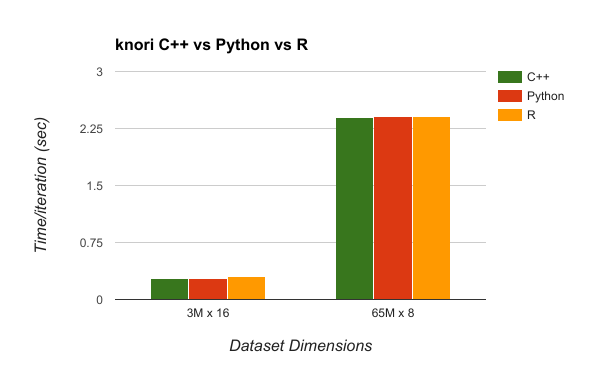
\includegraphics[width=.45\textwidth]{../../figs/binding-from-disk.png}
\caption{The performance of bindings when data are located on disk.}
\label{fig:bindings}
\end{cframed}
\end{figure}

\begin{figure}[!h]
\begin{cframed}
    \centering
    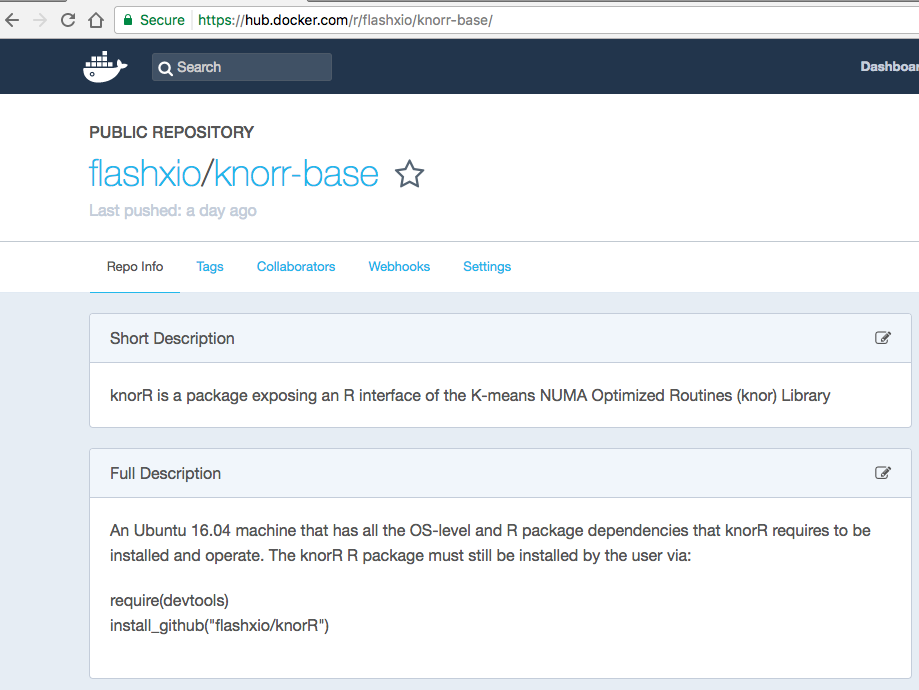
\includegraphics[width=.45\textwidth]{../../figs/binding-docker.png}
\caption{The docker hub base R image.}
\label{fig:binding-docker}
\end{cframed}
\end{figure}

\clearpage

\end{document}
